\section{The DYMO Protocol}
\label{sec:dymooverview}
The Dynamic MANET On-demand routing protocol is a routing protocol for \emph{mobile ad-hoc networks} (MANETs). It is currently under development by the IETF MANET working group \cite{RefWorks:89}. The specification is an Internet-draft \cite{RefWorks:88}, and is expected to become a Request for Comments (RFC) document in the near future.

\subsection{Mobile Ad-hoc Networks}
A MANET \cite{RefWorks:90} is a network consisting of mobile nodes, e.g., laptops, or mobile phones. The network has no pre-existing communication infrastructure in contrast to, e.g., WLANs where the nodes communicate with each other through a base station. The nodes in a MANET must therefore communicate directly with one another, i.e., send messages to those nodes that are within physical transmission range. This means, that it is the power of the radio, and the physical position of the nodes, that determine the topology of the network. The topology of the network may change rapidly because of node mobility, and links between nodes might disappear and reappear frequently. A typical use of MANETs is during emergency search-and-rescue operations in remote areas where no pre-existing communication infrastructure exists. 

\newpage

In order to communicate with nodes outside a given nodes physical range a routing protocol is needed to perform multi-hop communication, i.e., nodes forward data packets on behalf of other nodes in the network. The topology of a small MANET with five nodes is shown in Fig.~\ref{fig:topology}. An edge between two nodes indicates that the nodes are within direct transmission range of each other, e.g., node 1 is able to send messages directly to node 2 and node 3. 

\begin{figure}
\centering
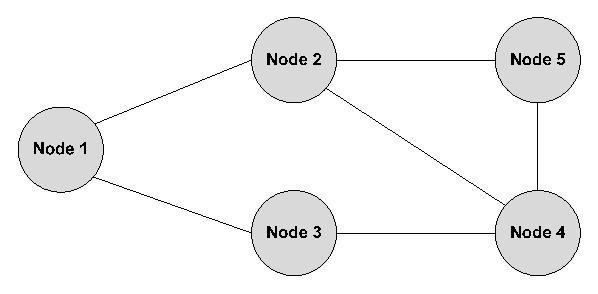
\includegraphics[scale=0.8]{dymo/graphics/topology_ex.eps}
\caption{Five node example topology}
\label{fig:topology}
\end{figure}

Routing protocols for MANETs are often categorised as being either \emph{proactive} or \emph{reactive}. The proactive routing protocols are constantly trying to keep an updated view of the network topology by maintaining a route to the other nodes in the network. The reactive routing protocols establish routes on demand, i.e., when routes are needed, and often do little maintenance on existing routes.

\subsection{The Operations of DYMO}
The DYMO routing protocol is a reactive protocol which establishes routes only when they are needed. The protocol has two main parts which are \emph{route discovery} and \emph{route maintenance}. Route maintenance is done by using active link monitoring and timeouts. If a node becomes aware that a route is broken it sends a \emph{Route Error} (RERR) message to the surrounding nodes, and thereby informs them that the route can no longer be used.

Route discovery is used to establish routes to other nodes in the network. An \emph{originator} node multicasts a \emph{Route Request} (RREQ) message which is sent hop-by-hop throughout the network to find a route to the \emph{target} node of the request. Each intermediate node records a route back to the originator node. When the target node receives the RREQ message it replies with a \emph{Route Reply} (RREP) message. This is unicasted back hop-by-hop towards the originator node using the routes recorded when the RREQ was sent. When the originator node receives the RREP message, the route has been established between the originator node and the target node in both directions.


\begin{figure}
\centering
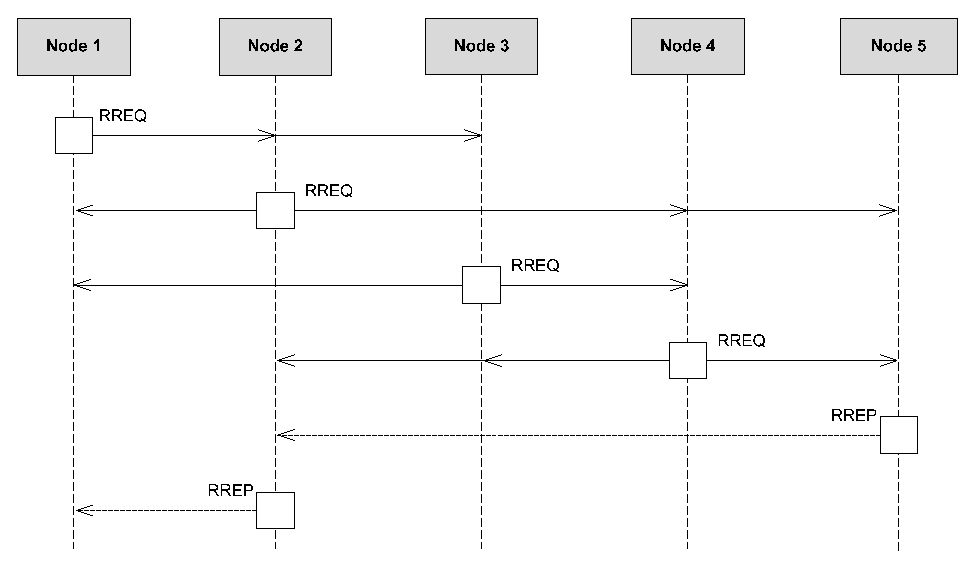
\includegraphics[width=\textwidth]{dymo/graphics/mscdymoex.eps}
\caption{Message sequence chart of a route request}
\label{fig:mscrreq}
\end{figure}

To get a better understanding of the protocol we present an example of how route discovery is performed in the small MANET shown in Fig.~\ref{fig:topology}. Fig.~\ref{fig:mscrreq} shows a message sequence chart (MSC) of one possible exchange of messages in the DYMO protocol when the originator node 1 is requesting a route to the target node 5. A solid arc represents multicast, and a dashed arc represents unicast. In the MSC, node 1 initiates the route request by multicasting a RREQ which is received by nodes 2 and 3. Node 2 and node 3 both records the route back to node 1 in their \emph{routing tables}, and then forwards the RREQ. Node 2 multicasts the RREQ message which is received by the nodes within transmission range, i.e., node 1, node 4, and node 5. Node 3 also multicasts the RREQ message which is received by node 1, and node 4. Node 1 discards the RREQs from node 2 and node 3 because it is the originator of the message. Node 4 first receives the RREQ from node 2 and records the route back to node 1. When node 4 receives the RREQ from node 3, it has already recorded a route to node 1 with the same length (number of hops) and the message is discarded.

Node 4 then multicasts the RREQ which is received by node 2, node 3, and node 5. The message is discarded by node 2 and node 3 since they already know of a shorter route to the originator node 1. Node 5 has received a RREQ from both node 2 and node 4, but since the RREQ from node 2 has a shorter route to node 1 this route is recorded in the routing table. Furthermore, node 5 is the target of the RREQ, and therefore replies with a RREP message with node 1 as the target. The RREP is unicasted back along the same route as the RREQ was sent which means that node 5 sends the RREP to node 2. When node 2 receives the RREP it already knows a route to node 1 (because of the RREQ) and unicasts the RREP to node 1. When node 1 receives the RREP a route is established between node 1 and node 5 in both directions.